\documentclass[a4paper,11pt]{article}
\usepackage{fullpage}
\usepackage{graphicx}
\usepackage{eqnarray,amsmath}


\pdfinfo{
/Title (ELEN3007-Assignment-2024)
/Author (Kgadile "Naar-Kie" Masemola)
/CreationDate (D:202303151636)
/ModDate (D:202409040530)
/Subject (ELEN3XXX Paper Format, 2024)
%/Keywords (ELEN3009, paper, project)
}

\title{ELEN3007A Group \underline{21} - Assignment 2024: \\ 
\large \emph{Application of Bayes’ Theorem for Locating a Robot’s
Position in an Enclosed Area}}
\author{Kgadile E Masemola (876729),  Thembinkosi Dhlamini (1234567),
 \\Siphokuhle Zulu (7654321), Lesego Gaborone (2176543)}
\date{September 13, 2024}

\begin{document}
\maketitle

\section*{Introduction and Background}
The assignment consideres that the position of $\beta$ is known, and after recording \emph{N} flashes at positions $x_k$, and inferes or answers the question: \emph{where is the robot}?\\
The azimuth angles at which the flashes are emmited, at random intervals, are quantified by $\theta_k$ which is uniformly distributed distributed. Since $\theta_k$ is uniformly distributed, we expect more recordings of $x_k$ near or around $\alpha$ which displays the vertical position underwhich the robot is expected to be. The mean value of $x_k$ is distance away from the assumed value of $\alpha$.

\subsection*{Assessment Criterion}
\begin{itemize}
	\item Geometry setup of the problem
		\begin{figure}[h]
        		\centering
        		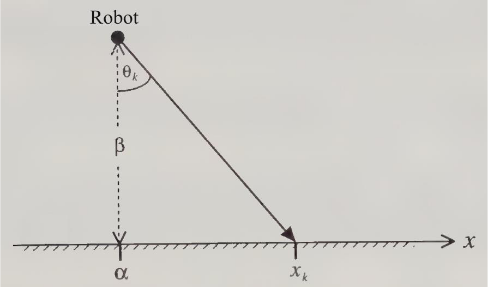
\includegraphics[scale=0.5]{elen3007assignfig.png} 
        		\caption{Geometry setup of the problem}
        \end{figure}
	\item $\theta_k$ assumed to be uniform, azimuth angles lying between $-\frac{\pi}{2}$ and $\frac{\pi}{2}$, it has the PDF:
		\begin{equation}
			p(\theta_k | \alpha, \beta, B) = \frac{1}{\pi}
		\end{equation}
	\item In order to relate the readings of $x_k$ to $\theta_k$, using elementary trigonometry, the derived expression is
		\begin{equation}
			\beta tan \theta_k = x_k - \alpha
		\end{equation}
\end{itemize}

\section*{Assignment Answers}
\begin{enumerate}
  \item The given setup of the problem assumes that the photodetectors are placed on the x-axis above which the robot is located. Therefore, the signal comes from one side of the axis. This thus limits the range of the detectors to be within the range of $\pi$ (that is $-\frac{\pi}{2}$ to $\frac{\pi}{2}$). 
  \item Second
  \item Etc.
\end{enumerate}

\section*{Conclusion}
\end{document}